\documentclass[14pt, a4paper]{extarticle}
\usepackage[T2A]{fontenc}
\usepackage[utf8]{inputenc}
\usepackage[english,russian]{babel}
\usepackage[left = 3cm, right = 1cm, top = 2cm, bottom = 2cm]{geometry}
\setlength\parindent{12.5mm} 
\linespread{1.3}
\usepackage{enumitem}
\usepackage{amsmath}
\usepackage{amssymb}
\usepackage{wrapfig}
\usepackage{indentfirst}
\usepackage{hyperref} % ДОЛЖЕН БЫТЬ ПОСЛЕДНИМ (кроме cleveref)
\hypersetup{
	colorlinks=true,
	citecolor=blue,
	urlcolor=blue, 
	linkcolor=blue,
	pdfencoding=auto
}
\usepackage{xcolor}   % Пакет для работы с цветами
\usepackage{listings} % Пакет для оформления кода
\usepackage{graphicx}
\usepackage{float}
\usepackage{longtable}
\usepackage[htt]{hyphenat}
% Определяем приглушенные цвета для академического стиля
\definecolor{codegreen}{rgb}{0,0.6,0}
\definecolor{codegray}{rgb}{0.5,0.5,0.5}
\definecolor{codepurple}{rgb}{0.58,0,0.82}
\definecolor{backcolour}{rgb}{0.97,0.97,0.97}
% Глобальная настройка стиля листингов
\lstset{ 
	language=C++,                       % Указываем язык по умолчанию
	backgroundcolor=\color{backcolour}, % Светло-серый фон
	commentstyle=\color{codegreen}\itshape, % Комментарии зеленым курсивом
	keywordstyle=\color{blue}\bfseries, % Ключевые слова синим и жирным
	numberstyle=\tiny\color{codegray},  % Стиль номеров строк (мелкий, серый)
	stringstyle=\color{codepurple},     % Строки фиолетовым
	basicstyle=\ttfamily\footnotesize,  % Моноширинный шрифт, чуть меньше основного
	breakatwhitespace=false,         
	breaklines=true,                    % Автоматический перенос длинных строк
	captionpos=t,                       % Позиция заголовка (t - сверху, b - снизу)
	keepspaces=true,                 
	numbers=left,                       % Номера строк слева
	numbersep=10pt,                     % Отступ номеров от кода
	showspaces=false,                
	showstringspaces=false,
	showtabs=false,                  
	tabsize=4,                          % Размер табуляции
	frame=single,                       % Одинарная рамка вокруг кода
	rulecolor=\color{black!30},          % Цвет рамки (светло-серый)
	extendedchars=\true
}
\newcommand{\tab}{\hspace{12.5mm}}

\usepackage{tabularx} % Обязательный пакет для этого способа

% Создаем команду для удобного центрирования текста внутри растягиваемых ячеек
\newcolumntype{Y}{>{\centering\arraybackslash}X}

\begin{document}
	\thispagestyle{empty}
	\begin{center}
		\hspace{0.2cm}МИНИСТЕРСТВО НАУКИ И ВЫСШЕГО ОБРАЗОВАНИЯ РОССИЙСКОЙ ФЕДЕРАЦИИ\\
		Федеральное государственное автономное образовательное\\
		учреждение высшего образования\\
		{\bf <<Санкт-Петербургский политехнический\\
			университет Петра Великого>>}\\
		Институт компьютерных наук и кибербезопасности\\
		Высшая школа технологий искусственного интеллекта\\
		02.03.01\_03 Технологии машинного обучения и искусственного интеллекта\\
		\vspace{3cm}
		\Large\bf{
			Отчёт о выполнении лабораторной работы №5\\
			Основы архитектуры ЦВМ\\[1cm]
		}
	\end{center}
	\vspace{2cm}
	\begin{flushleft}
		{\bf Выполнил:}\\
		Cтудент группы 5130201/50302 \hfill
		\line(1,0){4cm} \quad Калинский В.И.\\
		{\bf Принял:}\\
		К.т.н., доцент, доцент ВШТИИ и КОЦ ИИ \hfill
		\line(1,0){3 cm} \quad Вербова Н.М.\\[0.5cm]
		{ \hfill<<\rule{1cm}{0.5pt}>>\rule{2cm}{0.5pt}\hspace{3pt}2026 г.}
	\end{flushleft}
	\vspace{1cm}
	\begin{center}
		Санкт-Петербург, 2026
	\end{center}
	\newpage
	\noindent \textbf{Цель работы:}
	
	Изучить принципы действия цифро-аналоговых и аналого-цифровых
	преобразователей.
	\\\\
	\noindent \textbf{Методика:}
	
	В первой части работы необходимо синтезировать двухразрядный АЦП параллельного преобразования ($n = 2$). Число уровней квантования равно $2^n = 4$, для различения которых требуется $2^n - 1 = 3$ компаратора ($K_1, K_2, K_3$) для трёх границ состояний и прецизионный резистивный делитель напряжения.
	
	Нижнее и верхнее сопротивления выбираются равными $R_n = R/2$, а два промежуточных -- равными $R$. Примем $R = 1\text{ кОм}$ (тогда $R/2 = 500\text{ Ом}$) и опорное напряжение $U_{\text{оп}} = 3\text{ В}$ (шаг квантования $h = 1\text{ В}$). Суммарное сопротивление делителя составляет $R_{\Sigma} = 0{,}5 + 1 + 1 + 0{,}5 = 3\text{ кОм}$, ток делителя $I = U_{\text{оп}}/R_{\Sigma} = 1\text{ мА}$. Пороговое напряжение на инвертирующем входе $k$-го компаратора равно падению напряжения на участке делителя между соответствующим узлом и землёй:
	\begin{equation*}
		U_{\text{пор}\,k} = I \cdot R_{\text{ниже}\,k},
	\end{equation*}
	откуда:
	\begin{align*}
		U_{\text{пор1}} &= 0{,}5\text{ В}, & U_{\text{пор2}} &= 1{,}5\text{ В}, & U_{\text{пор3}} &= 2{,}5\text{ В}.
	\end{align*}
	
	Сигналы с выходов компараторов фиксируются в $D$-триггерах по сигналу «Запуск» (выходы триггеров обозначим $Q_3, Q_2, Q_1$ от старшего порога к младшему) и поступают на приоритетный шифратор (таблица \ref{tab:flash_enc}).
	
	\begin{table}[H]
		\centering
		\begin{tabular}{|c|c|c|c|c|c|c|}
			\hline
			Диапазон $U_{\text{вх}}$, В & Десятичный экв. & $Q_3$ & $Q_2$ & $Q_1$ & $Z_1$ & $Z_0$ \\ \hline
			$0 \le U_{\text{вх}} < 0{,}5$ & 0 & 0 & 0 & 0 & 0 & 0 \\ \hline
			$0{,}5 < U_{\text{вх}} < 1{,}5$ & 1 & 0 & 0 & 1 & 0 & 1 \\ \hline
			$1{,}5 < U_{\text{вх}} < 2{,}5$ & 2 & 0 & 1 & 1 & 1 & 0 \\ \hline
			$U_{\text{вх}} > 2{,}5$ & 3 & 1 & 1 & 1 & 1 & 1 \\ \hline
		\end{tabular}
		\caption{Таблица состояний компараторов и приоритетного шифратора}
		\label{tab:flash_enc}
	\end{table}
	
	
	По рабочим наборам таблицы \ref{tab:flash_enc} запишем совершенную дизъюнктивную нормальную форму (СДНФ) для выходов $Z_1$ и $Z_0$:
	\begin{align*}
		Z_1 &= \overline{Q}_3 Q_2 Q_1 + Q_3 Q_2 Q_1, \\
		Z_0 &= \overline{Q}_3 \overline{Q}_2 Q_1 + Q_3 Q_2 Q_1.
	\end{align*}
	
	На основе таблицы истинности построим карты Карно для функций $Z_1$ и $Z_0$ от трёх переменных $(Q_3, Q_2, Q_1)$. Жирным шрифтом выделены контуры склеивания.
	
	\begin{center}
		\small
		\begin{minipage}{0.48\textwidth}
			\centering
			\textbf{Карта Карно для $Z_1$}\\[4pt]
			\begin{tabular}{|c|c|c|c|c|}
				\hline
				& $Q_2 Q_1$ & $Q_2 \overline{Q}_1$ & $\overline{Q}_2 \overline{Q}_1$ & $\overline{Q}_2 Q_1$ \\ \hline
				$Q_3$            & \textbf{1} & \textbf{*} & * & * \\ \hline
				$\overline{Q}_3$ & \textbf{1} & \textbf{*} & 0 & 0 \\ \hline
			\end{tabular}
		\end{minipage}
		\hfill
		\begin{minipage}{0.48\textwidth}
			\centering
			\textbf{Карта Карно для $Z_0$}\\[4pt]
			\begin{tabular}{|c|c|c|c|c|}
				\hline
				& $Q_2 Q_1$ & $Q_2 \overline{Q}_1$ & $\overline{Q}_2 \overline{Q}_1$ & $\overline{Q}_2 Q_1$ \\ \hline
				$Q_3$            & \textbf{1} & \textbf{*} & \textbf{*} & \textbf{*} \\ \hline
				$\overline{Q}_3$ & 0 & * & 0 & \textbf{1} \\ \hline
			\end{tabular}
		\end{minipage}
	\end{center}
	
	Минимизация с помощью карт Карно даёт:
	$Z_1 = Q_2.$
	$Z_0 = Q_3 + \overline{Q}_2 Q_1.$
	
	Таким образом, старший разряд $Z_1$ снимается непосредственно с выхода второго триггера $Q_2$, а для формирования младшего разряда $Z_0$ используется один двухвходовый элемент И и один двухвходовый элемент ИЛИ. Синтезированная схема 2-разрядного АЦП параллельного преобразования в среде Multisim представлена на рис. \ref{fig:5-1}.
	
	\begin{figure}[H]
		\centering
		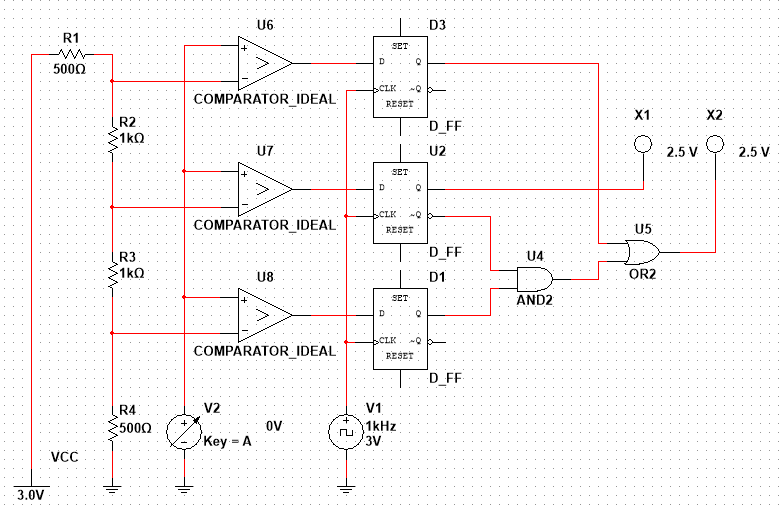
\includegraphics[width=0.85\linewidth]{5-1}
		\caption{Принципиальная схема 2-разрядного АЦП параллельного преобразования в Multisim}
		\label{fig:5-1}
	\end{figure}
	
	Во второй части работы необходимо синтезировать двухразрядный АЦП последовательного приближения. Структурно устройство включает в себя компаратор, двухразрядный ЦАП, устройство управления и регистр последовательного приближения (РПП). Далее приведены синтезы каждой из частей.
	
	Было синтезировано устройство управления, формирующее стробирующие импульсы $T_1$, $T_2$, $T_3$. Распределитель строится на базе трёх тактируемых $D$-триггеров ($Q_1, Q_2, Q_3$), где:
	\begin{align*}
		T_1 &= Q_1, & T_2 &= Q_2, & T_3 &= Q_3.
	\end{align*}
	
	Последовательность смены состояний распределителя задаётся циклическим переходом:
	\begin{equation*}
		100 \longrightarrow 010 \longrightarrow 001 \longrightarrow 100.
	\end{equation*}
	
	Поскольку 3 триггера имеют $2^3 = 8$ состояний, 5 состояний являются неиспользуемыми ($000, 011, 101, 110, 111$). Составим таблицу переходов и функций возбуждения входов $D_1, D_2, D_3$ с учётом того, что для $D$-триггера $D_i = Q_i^{t+1}$ (таблица \ref{tab:distr_trans}).
	
	\begin{table}[H]
		\centering
		\begin{tabular}{|c|c|c|c|c|c|c|}
			\hline
			$Q_1^t$ & $Q_2^t$ & $Q_3^t$ & $Q_1^{t+1}$ & $Q_2^{t+1}$ & $Q_3^{t+1}$ & Такт \\ \hline
			1 & 0 & 0 & 0 & 1 & 0 & $T_1 = 1$ \\ \hline
			0 & 1 & 0 & 0 & 0 & 1 & $T_2 = 1$ \\ \hline
			0 & 0 & 1 & 1 & 0 & 0 & $T_3 = 1$ \\ \hline
		\end{tabular}
		\caption{Таблица переходов и функций возбуждения 3-фазного распределителя тактов}
		\label{tab:distr_trans}
	\end{table}
	
	На основе таблицы переходов построим карты Карно для $D_1, D_2, D_3$ распределителя тактов. Жирным шрифтом выделены контуры склеивания.
	
	\begin{center}
		\small
		\begin{minipage}{0.32\textwidth}
			\centering
			\textbf{$D_1$}\\[4pt]
			\begin{tabular}{|c|c|c|c|c|}
				\hline
				& $Q_2 Q_3$ & $Q_2 \overline{Q}_3$ & $\overline{Q}_2 \overline{Q}_3$ & $\overline{Q}_2 Q_3$ \\ \hline
				$Q_1$            & 0 & 0 & 0 & 0 \\ \hline
				$\overline{Q}_1$ & 0 & 0 & \textbf{1} & \textbf{1} \\ \hline
			\end{tabular}
		\end{minipage}
		\hfill
		\begin{minipage}{0.32\textwidth}
			\centering
			\textbf{$D_2$}\\[4pt]
			\begin{tabular}{|c|c|c|c|c|}
				\hline
				& $Q_2 Q_3$ & $Q_2 \overline{Q}_3$ & $\overline{Q}_2 \overline{Q}_3$ & $\overline{Q}_2 Q_3$ \\ \hline
				$Q_1$            & \textbf{*} & \textbf{*} & \textbf{1} & \textbf{*} \\ \hline
				$\overline{Q}_1$ & 0 & 0 & 0 & 0 \\ \hline
			\end{tabular}
		\end{minipage}\\
		\begin{minipage}{0.32\textwidth}
			\centering
			\textbf{$D_3$}\\[4pt]
			\begin{tabular}{|c|c|c|c|c|}
				\hline
				& $Q_2 Q_3$ & $Q_2 \overline{Q}_3$ & $\overline{Q}_2 \overline{Q}_3$ & $\overline{Q}_2 Q_3$ \\ \hline
				$Q_1$            & \textbf{*} & \textbf{*} & 0 & 0 \\ \hline
				$\overline{Q}_1$ & \textbf{*} & \textbf{1} & 0 & 0 \\ \hline
			\end{tabular}
		\end{minipage}
	\end{center}
	
	По результатам минимизации карт Карно получаем уравнения входов возбуждения:
	\begin{align*}
		D_1 &= \overline{Q}_1 \overline{Q}_2 \overline{Q}_3 + \overline{Q}_1 \overline{Q}_2 Q_3 = \overline{Q}_1 \overline{Q}_2 = \overline{Q_1 + Q_2}, \\
		D_2 &= Q_1, \\
		D_3 &= Q_2.
	\end{align*}
	
	Далее синтезируем блок памяти 2-разрядного АЦП последовательного приближения, построенный на двух тактируемых $D$-триггерах: старшего разряда $Z_1$ (СЗР) и младшего разряда $Z_0$ (МЗР).
	
	Регистр управляется трёхфазным распределителем тактов ($T_1, T_2, T_3$) и логическим сигналом с выхода компаратора $K$, где:
	\begin{equation*}
		K = \begin{cases} 
			1, & \text{если } U_{\text{вх}} \ge U_{\text{ЦАП}} \text{ (пробный разряд подтверждается)}, \\ 
			0, & \text{если } U_{\text{вх}} < U_{\text{ЦАП}} \text{ (пробный разряд сбрасывается)}. 
		\end{cases}
	\end{equation*}
	
	Функционирование регистра подчиняется следующему пошаговому алгоритму:
	\begin{enumerate}
		\item \textbf{Такт $T_1$ (Инициализация и пробный вес СЗР):} в регистр принудительно заносится код $Z_1 = 1$, $Z_0 = 0$. ЦАП вырабатывает напряжение половины шкалы $U_{\text{ЦАП}} = 2{,}5\text{ В}$, а компаратор формирует сигнал решения по старшему разряду $K_1$.
		\item \textbf{Такт $T_2$ (Фиксация СЗР и пробный вес МЗР):} в старший разряд записывается результат первого сравнения ($Z_1 = K_1$), а в младший разряд принудительно выставляется единица ($Z_0 = 1$). ЦАП формирует напряжение второй ступени, а компаратор формирует решение по младшему разряду $K_2$.
		\item \textbf{Такт $T_3$ (Фиксация МЗР и сохранение кода):} старший разряд сохраняет значение ($Z_1 = K_1$), а в младший разряд записывается результат второго сравнения ($Z_0 = K_2$). На выходах $(Z_1, Z_0)$ устанавливается устойчивый двоичный эквивалент входного напряжения.
	\end{enumerate}
	
	Составим таблицу переходов регистра памяти по тактам (таблица \ref{tab:sar_mem_trans}). В такте $T_3$ старший разряд должен сохранять значение, поэтому для него $Z_1^{t+1} = Z_1^t$.
	
	\begin{table}[H]
		\centering
		\begin{tabular}{|c|c|c|c|}
			\hline
			Активный такт & $Z_1^{t+1}$ & $Z_0^{t+1}$ & Код на выходе ЦАП \\ \hline
			$T_1$ & 1 & 0 & $10_2$ \\ \hline
			$T_2$ & $K_1$ & 1 & $K_1 1_2$ \\ \hline
			$T_3$ & $Z_1^t$ & $K_2$ & $K_1 K_2$ \\ \hline
		\end{tabular}
		\caption{Таблица переходов регистра последовательного приближения (РПП)}
		\label{tab:sar_mem_trans}
	\end{table}
	
	Для $D$-триггера $D = Q^{t+1}$, поэтому по таблице получаем уравнения входов:
	\begin{align*}
		D_{Z1} &= T_1 + T_2 K + T_3 Z_1, \\
		D_{Z0} &= T_2 + T_3 K.
	\end{align*}
	В такте $T_1$ оба слагаемых $D_{Z0}$ равны нулю, поэтому $Z_0$ сбрасывается в ноль без отдельного сигнала сброса.
	
	Далее синтезирован 2-разрядный ЦАП на базе резистивной матрицы лестничного типа $R$--$2R$.
	
	Для преобразования промежуточного кода регистра памяти в компенсирующее аналоговое напряжение $U_{\text{ЦАП}}$ используется двухразрядный цифро-аналоговый преобразователь (ЦАП) на резистивной матрице лестничного типа $R$--$2R$.
	
	Матрица состоит из резисторов двух номиналов: $R = 10\text{ кОм}$ и $2R = 20\text{ кОм}$. Входными сигналами служат логические уровни с прямых выходов триггеров памяти $Z_1$ и $Z_0$. Логической единице соответствует потенциал питания $V_{CC} = 5\text{ В}$, логическому нулю — потенциал земли $0\text{ В}$.
	
	Рассчитаем вклад каждого разряда в выходное напряжение $U_{\text{ЦАП}}$ методом наложения:
	\begin{enumerate}
		\item \textbf{Вклад младшего разряда ($Z_1 = 0$, $Z_0 = 1$):} ветвь $Z_0$ ($2R$ к $V_{CC}$) и согласующий резистор ($2R$ на землю) образуют делитель, эквивалентный генератору с ЭДС $U_A = V_{CC}/2$ и внутренним сопротивлением $2R \parallel 2R = R$. Этот генератор через продольный резистор $R$ нагружен на выходной узел, к которому подключена заземлённая ветвь старшего разряда ($2R$). Последовательная цепь $R + R = 2R$ и сопротивление $2R$ ветви $Z_1$ образуют делитель пополам:
		\begin{equation*}
			U_{\text{ЦАП}}(Z_0) = \frac{U_A}{2} = \frac{V_{CC}}{4} = 1{,}25\text{ В}.
		\end{equation*}
		\item \textbf{Вклад старшего разряда ($Z_1 = 1$, $Z_0 = 0$):} напряжение $V_{CC}$ приложено к ветви $Z_1$. Вся левая часть схемы (цепь младшего разряда с согласующим резистором) имеет эквивалентное входное сопротивление $R_{\text{экв}} = R + (2R \parallel 2R) = 2R$. Напряжение на выходе делится между ветвью $Z_1$ ($2R$) и левой частью ($2R$) строго пополам:
		\begin{equation*}
			U_{\text{ЦАП}}(Z_1) = \frac{V_{CC}}{2} = 2{,}50\text{ В}.
		\end{equation*}
	\end{enumerate}
	
	Результирующее выходное напряжение ЦАП описывается линейной суперпозицией:
	\begin{equation*}
		U_{\text{ЦАП}} = \frac{V_{CC}}{4} (2 Z_1 + Z_0) = 1{,}25\text{ В} \cdot (2 Z_1 + Z_0).
	\end{equation*}
	
	Зависимость выходного напряжения от состояния разрядов памяти представлена в таблице \ref{tab:dac_levels}.
	
	\begin{table}[H]
		\centering
		\begin{tabular}{|c|c|c|c|}
			\hline
			Код $(Z_1 Z_0)$ & Цифра & Аналитическое выражение & Напряжение $U_{\text{ЦАП}}$, В \\ \hline
			$00_2$ & 0 & $0$ & $0{,}00$ \\ \hline
			$01_2$ & 1 & $\frac{1}{4} V_{CC}$ & $1{,}25$ \\ \hline
			$10_2$ & 2 & $\frac{2}{4} V_{CC}$ & $2{,}50$ \\ \hline
			$11_2$ & 3 & $\frac{3}{4} V_{CC}$ & $3{,}75$ \\ \hline
		\end{tabular}
		\caption{Выходные уровни напряжения 2-разрядного ЦАП с матрицей $R$--$2R$}
		\label{tab:dac_levels}
	\end{table}
	
	Схема АЦП последовательного приближения, собранная в Multisim, приведена на рис. \ref{fig:5-2}. 
	
	\begin{figure}[H]
		\centering
		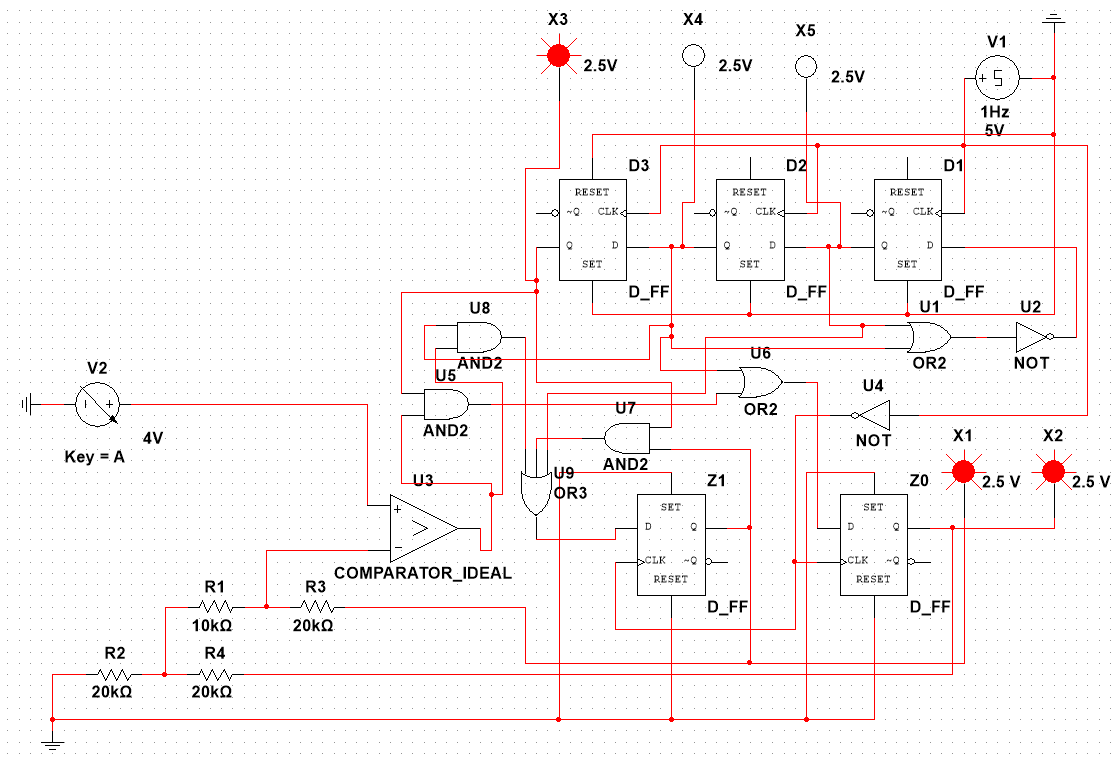
\includegraphics[width=0.95\linewidth]{5-2}
		\caption{Принципиальная схема 2-разрядного АЦП последовательного приближения в Multisim}
		\label{fig:5-2}
	\end{figure}
	
	\noindent \textbf{Выводы:}
	
	В ходе выполнения лабораторной работы были изучены принципы действия аналого-цифровых преобразователей. Синтезирован и исследован двухразрядный АЦП параллельного преобразования на трёх компараторах. По картам Карно получены уравнения $Z_1 = Q_2$ и $Z_0 = Q_3 + \overline{Q}_2 Q_1$, схема содержит один элемент И и один ИЛИ. Синтезирован и исследован двухразрядный АЦП последовательного приближения: распределитель тактов на трёх $D$-триггерах, регистр на двух $D$-триггерах с входами $D_{Z1} = T_1 + T_2 K + T_3 Z_1$, $D_{Z0} = T_2 + T_3 K$ и ЦАП на матрице $R$--$2R$ с уровнями $0$; $1{,}25$; $2{,}5$; $3{,}75\text{ В}$. 
	
	%КАРТИНКИ
	%\begin{figure}[H]
	%	\centering
	%	\includegraphics[width=0.85\textwidth]{install_deb.png}
	%	\caption{Начало установки гостевой ОС Debian 12}
	%	\label{fig:vbox_setup}
	%\end{figure}
	
	%---------------------------------------------------------------------------------
	%ССЫЛКИ НА САЙТ
	
	%\href{https://www.virtualbox.org/wiki/Downloads}{официального сайта VirtualBox}
	
	%---------------------------------------------------------------------------------
	%ССЫЛКА НА ПРИЛОЖЕНИЕ
	
	%\texttt{zlib}\cite{zlib_docs}
	
	%---------------------------------------------------------------------------------
	%ССЫЛКА НА РИСУНОК
	
	%показано на рис. \ref{fig:vbox_setup}
	
	%---------------------------------------------------------------------------------
	%ТАБЛИЦА С ПЕРЕВОДОМ НА СЛЕДУЮЩУЮ СТРАНИЦУ
	
	%\begin{longtable}{|l|p{0.75\textwidth}|}
	%	\caption{Функции библиотеки ncurses, используемые в TUI} \label{tab:ncurses_funcs} \\
	%	\hline
	%	\textbf{Функция} & \textbf{Назначение и описание алгоритма работы} \\ \hline
	%	\endhead
	%	\texttt{initscr()} & Инициализирует библиотеку, выделяет память под внутренние структуры окна и переводит терминал ОС в графический режим. \\ \hline
	%	\texttt{cbreak()} & Отключает строковую буферизацию терминала, позволяя программе мгновенно реагировать на нажатия клавиш без ожидания \texttt{Enter}. \\ \hline
	%	\texttt{noecho()} & Отключает автоматический вывод (эхо) вводимых пользователем символов на экран, позволяя программе самой управлять отрисовкой. \\ \hline
	%	\texttt{clear()} & Очищает виртуальный экран для подготовки к отрисовке нового кадра меню. \\ \hline
	%	\texttt{move(y, x)} & Осуществляет абсолютное позиционирование курсора по координатам \texttt{Y} (строка) и \texttt{X} (столбец). \\ \hline
	%	\texttt{printw()} & Аналог функции \texttt{printf} для \texttt{ncurses}: выводит отформатированный текст в текущей позиции курсора. \\ \hline
	%	\texttt{getch()} & Ожидает и считывает код нажатой пользователем клавиши (включая стрелки навигации и функциональные клавиши). \\ \hline
	%	\texttt{getnstr()} & Безопасно считывает строку от пользователя с аппаратным ограничением максимального количества символов (защита от переполнения). \\ \hline
	%	\texttt{scanw()} & Аналог функции \texttt{scanf}, считывает форматированный ввод пользователя (применяется для ввода числовых данных). \\ \hline
	%	\texttt{endwin()} & Выгружает библиотеку из памяти, восстанавливает историю команд и возвращает терминал в стандартный режим работы ОС. \\ \hline
	%\end{longtable}
	%---------------------------------------------------------------------------------
	
\end{document}